\documentclass[twoside]{book}

% Packages required by doxygen
\usepackage{fixltx2e}
\usepackage{calc}
\usepackage{doxygen}
\usepackage[export]{adjustbox} % also loads graphicx
\usepackage{graphicx}
\usepackage[utf8]{inputenc}
\usepackage{makeidx}
\usepackage{multicol}
\usepackage{multirow}
\PassOptionsToPackage{warn}{textcomp}
\usepackage{textcomp}
\usepackage[nointegrals]{wasysym}
\usepackage[table]{xcolor}

% Font selection
\usepackage[T1]{fontenc}
\usepackage[scaled=.90]{helvet}
\usepackage{courier}
\usepackage{amssymb}
\usepackage{sectsty}
\renewcommand{\familydefault}{\sfdefault}
\allsectionsfont{%
  \fontseries{bc}\selectfont%
  \color{darkgray}%
}
\renewcommand{\DoxyLabelFont}{%
  \fontseries{bc}\selectfont%
  \color{darkgray}%
}
\newcommand{\+}{\discretionary{\mbox{\scriptsize$\hookleftarrow$}}{}{}}

% Page & text layout
\usepackage{geometry}
\geometry{%
  a4paper,%
  top=2.5cm,%
  bottom=2.5cm,%
  left=2.5cm,%
  right=2.5cm%
}
\tolerance=750
\hfuzz=15pt
\hbadness=750
\setlength{\emergencystretch}{15pt}
\setlength{\parindent}{0cm}
\setlength{\parskip}{3ex plus 2ex minus 2ex}
\makeatletter
\renewcommand{\paragraph}{%
  \@startsection{paragraph}{4}{0ex}{-1.0ex}{1.0ex}{%
    \normalfont\normalsize\bfseries\SS@parafont%
  }%
}
\renewcommand{\subparagraph}{%
  \@startsection{subparagraph}{5}{0ex}{-1.0ex}{1.0ex}{%
    \normalfont\normalsize\bfseries\SS@subparafont%
  }%
}
\makeatother

% Headers & footers
\usepackage{fancyhdr}
\pagestyle{fancyplain}
\fancyhead[LE]{\fancyplain{}{\bfseries\thepage}}
\fancyhead[CE]{\fancyplain{}{}}
\fancyhead[RE]{\fancyplain{}{\bfseries\leftmark}}
\fancyhead[LO]{\fancyplain{}{\bfseries\rightmark}}
\fancyhead[CO]{\fancyplain{}{}}
\fancyhead[RO]{\fancyplain{}{\bfseries\thepage}}
\fancyfoot[LE]{\fancyplain{}{}}
\fancyfoot[CE]{\fancyplain{}{}}
\fancyfoot[RE]{\fancyplain{}{\bfseries\scriptsize Generated by Doxygen }}
\fancyfoot[LO]{\fancyplain{}{\bfseries\scriptsize Generated by Doxygen }}
\fancyfoot[CO]{\fancyplain{}{}}
\fancyfoot[RO]{\fancyplain{}{}}
\renewcommand{\footrulewidth}{0.4pt}
\renewcommand{\chaptermark}[1]{%
  \markboth{#1}{}%
}
\renewcommand{\sectionmark}[1]{%
  \markright{\thesection\ #1}%
}

% Indices & bibliography
\usepackage{natbib}
\usepackage[titles]{tocloft}
\setcounter{tocdepth}{3}
\setcounter{secnumdepth}{5}
\makeindex

% Custom commands
\newcommand{\clearemptydoublepage}{%
  \newpage{\pagestyle{empty}\cleardoublepage}%
}

\usepackage{caption}
\captionsetup{labelsep=space,justification=centering,font={bf},singlelinecheck=off,skip=4pt,position=top}

%===== C O N T E N T S =====

\begin{document}

% Titlepage & ToC
\pagenumbering{alph}
\begin{titlepage}
\vspace*{7cm}
\begin{center}%
{\Large key safe \\[1ex]\large 0.\+1 }\\
\vspace*{1cm}
{\large Generated by Doxygen 1.8.13}\\
\end{center}
\end{titlepage}
\clearemptydoublepage
\pagenumbering{roman}
\tableofcontents
\clearemptydoublepage
\pagenumbering{arabic}

%--- Begin generated contents ---
\chapter{File Index}
\section{File List}
Here is a list of all files with brief descriptions\+:\begin{DoxyCompactList}
\item\contentsline{section}{\textbf{ keysafe\+\_\+app.\+c} \\*File containing the main of the key safe application }{\pageref{keysafe__app_8c}}{}
\end{DoxyCompactList}

\chapter{File Documentation}
\section{keysafe\+\_\+app.\+c File Reference}
\label{keysafe__app_8c}\index{keysafe\+\_\+app.\+c@{keysafe\+\_\+app.\+c}}


File containing the main of the key safe application.  


{\ttfamily \#include $<$util/delay.\+h$>$}\newline
{\ttfamily \#include \char`\"{}../../utils/custom\+\_\+types.\+h\char`\"{}}\newline
{\ttfamily \#include \char`\"{}../../hal/lcd/lcd.\+h\char`\"{}}\newline
{\ttfamily \#include \char`\"{}../../hal/keypad/keypad.\+h\char`\"{}}\newline
{\ttfamily \#include \char`\"{}../../mcal/\+E\+E\+P\+R\+O\+M/eeprom.\+h\char`\"{}}\newline
Include dependency graph for keysafe\+\_\+app.\+c\+:\nopagebreak
\begin{figure}[H]
\begin{center}
\leavevmode
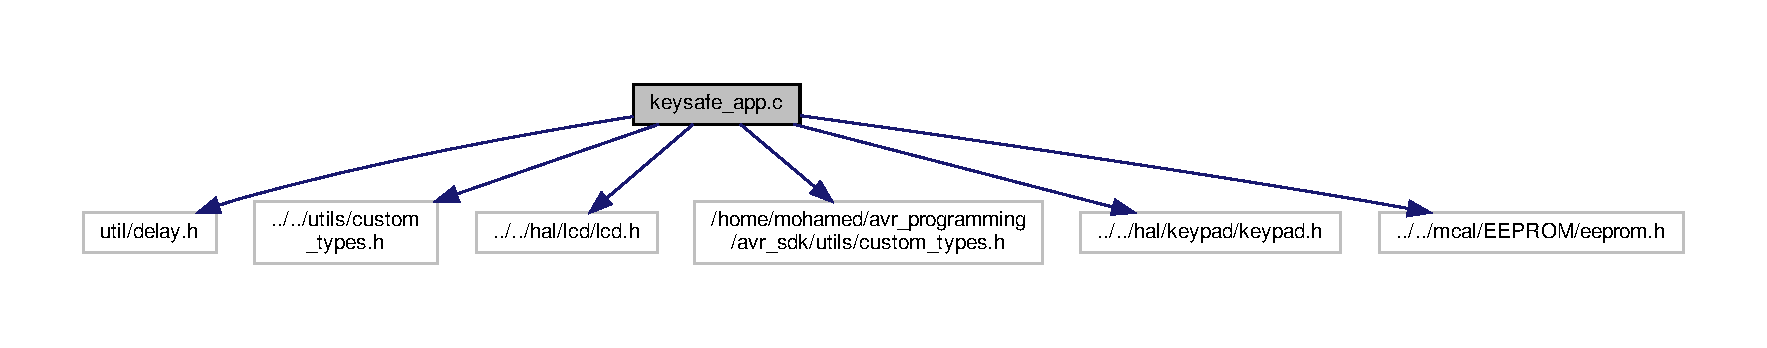
\includegraphics[width=350pt]{keysafe__app_8c__incl}
\end{center}
\end{figure}
\subsection*{Macros}
\begin{DoxyCompactItemize}
\item 
\#define \textbf{ P\+A\+S\+S\+W\+O\+R\+D\+\_\+\+E\+X\+I\+S\+T\+E\+D\+\_\+\+E\+E\+P\+R\+O\+M\+\_\+\+A\+DD}~0
\item 
\#define \textbf{ P\+A\+S\+S\+W\+O\+R\+D\+\_\+\+L\+E\+N\+G\+T\+H\+\_\+\+E\+E\+P\+R\+O\+M\+\_\+\+A\+DD}~1
\item 
\#define \textbf{ F\+I\+R\+S\+T\+\_\+\+D\+I\+G\+I\+T\+\_\+\+E\+E\+P\+R\+O\+M\+\_\+\+A\+DD}~2
\item 
\#define \textbf{ P\+A\+S\+S\+W\+O\+R\+D\+\_\+\+I\+N\+S\+E\+R\+T\+E\+D\+\_\+\+B\+Y\+T\+E\+\_\+\+V\+A\+L\+UE}~0x\+E0
\end{DoxyCompactItemize}
\subsection*{Functions}
\begin{DoxyCompactItemize}
\item 
void \textbf{ init\+\_\+system} (void)
\begin{DoxyCompactList}\small\item\em this function will initialize the whole system 1-\/initialize lcd 2-\/initialize keypad 3-\/initialize eeprom \end{DoxyCompactList}\item 
bool\+\_\+t \textbf{ is\+\_\+this\+\_\+new\+\_\+safe} (void)
\begin{DoxyCompactList}\small\item\em this function will check whether the user have entered the password for the save before or not by reading the eeprom P\+A\+S\+S\+W\+O\+R\+D\+\_\+\+E\+X\+I\+S\+T\+E\+D\+\_\+\+E\+E\+P\+R\+O\+M\+\_\+\+A\+DD and check whether it contains P\+A\+S\+S\+W\+O\+R\+D\+\_\+\+I\+N\+S\+E\+R\+T\+E\+D\+\_\+\+B\+Y\+T\+E\+\_\+\+V\+A\+L\+UE or not \end{DoxyCompactList}\item 
void \textbf{ enter\+\_\+new\+\_\+password\+\_\+handeller} (void)
\begin{DoxyCompactList}\small\item\em it handles the process of entering new password as follow 1-\/ ask user to enter new password 2-\/ wait user to hit enter 3-\/ store the password on E\+E\+P\+R\+OM strartino from addresss F\+I\+R\+S\+T\+\_\+\+D\+I\+G\+I\+T\+\_\+\+E\+E\+P\+R\+O\+M\+\_\+\+A\+DD 4-\/ update both P\+A\+S\+S\+W\+O\+R\+D\+\_\+\+L\+E\+N\+G\+T\+H\+\_\+\+E\+E\+P\+R\+O\+M\+\_\+\+A\+DD and P\+A\+S\+S\+W\+O\+R\+D\+\_\+\+E\+X\+I\+S\+T\+E\+D\+\_\+\+E\+E\+P\+R\+O\+M\+\_\+\+A\+DD \end{DoxyCompactList}\item 
u8\+\_\+t \textbf{ load\+\_\+save\+\_\+configuration} (u8\+\_\+t $\ast$pass\+\_\+container)
\item 
bool\+\_\+t \textbf{ scan\+\_\+save\+\_\+password} (u8\+\_\+t $\ast$entered\+\_\+digits, u8\+\_\+t $\ast$no\+\_\+of\+\_\+digits\+\_\+entered)
\begin{DoxyCompactList}\small\item\em it handles the process of entering password as follow 1-\/ ask user to enter password 2-\/ scan the user input and store it in entered\+\_\+digits at no\+\_\+of\+\_\+digits\+\_\+entered 3-\/ update the screen  entered\+\_\+digits\+:the address of a container to load the pressed key into it  no\+\_\+of\+\_\+digits\+\_\+entered \+: reference to a variable that stores how many digits are enter so far \end{DoxyCompactList}\item 
bool\+\_\+t \textbf{ is\+\_\+passwords\+\_\+equal} (u8\+\_\+t $\ast$entered\+\_\+digits, u8\+\_\+t $\ast$saved\+\_\+digits, u8\+\_\+t no\+\_\+of\+\_\+digits)
\begin{DoxyCompactList}\small\item\em it campares two arrays  entered\+\_\+digits\+:first array  saved\+\_\+digits \+: second array  no\+\_\+of\+\_\+digits \+: no of digits on each array \end{DoxyCompactList}\item 
void \textbf{ key\+\_\+safe\+\_\+app} (void)
\end{DoxyCompactItemize}


\subsection{Detailed Description}
File containing the main of the key safe application. 

\begin{DoxyAuthor}{Author}
Mohamed Yehia 
\end{DoxyAuthor}
\begin{DoxyDate}{Date}
Jul 20, 2019 
\end{DoxyDate}
\begin{DoxySeeAlso}{See also}
{\tt http\+://www.\+google.\+com} for more information regards of the project. the program stored the user password and some configuration on the E\+E\+P\+R\+OM as follow E\+E\+P\+R\+OM A\+D\+D\+R\+E\+SS 0 \+: contain whether the save has opened before or not(0xe0 mean it\textquotesingle{}s opened before) E\+E\+P\+R\+OM A\+D\+D\+R\+E\+SS 1 \+: contain the number of stored password length (8 if the password is 8 digits) E\+E\+P\+R\+OM A\+D\+D\+R\+E\+SS 2 \+: the first digit of the stored password 
\end{DoxySeeAlso}


\subsection{Macro Definition Documentation}
\mbox{\label{keysafe__app_8c_afccca8328f4f14d4aebfb6b9346701ee}} 
\index{keysafe\+\_\+app.\+c@{keysafe\+\_\+app.\+c}!F\+I\+R\+S\+T\+\_\+\+D\+I\+G\+I\+T\+\_\+\+E\+E\+P\+R\+O\+M\+\_\+\+A\+DD@{F\+I\+R\+S\+T\+\_\+\+D\+I\+G\+I\+T\+\_\+\+E\+E\+P\+R\+O\+M\+\_\+\+A\+DD}}
\index{F\+I\+R\+S\+T\+\_\+\+D\+I\+G\+I\+T\+\_\+\+E\+E\+P\+R\+O\+M\+\_\+\+A\+DD@{F\+I\+R\+S\+T\+\_\+\+D\+I\+G\+I\+T\+\_\+\+E\+E\+P\+R\+O\+M\+\_\+\+A\+DD}!keysafe\+\_\+app.\+c@{keysafe\+\_\+app.\+c}}
\subsubsection{F\+I\+R\+S\+T\+\_\+\+D\+I\+G\+I\+T\+\_\+\+E\+E\+P\+R\+O\+M\+\_\+\+A\+DD}
{\footnotesize\ttfamily \#define F\+I\+R\+S\+T\+\_\+\+D\+I\+G\+I\+T\+\_\+\+E\+E\+P\+R\+O\+M\+\_\+\+A\+DD~2}



Definition at line 20 of file keysafe\+\_\+app.\+c.

\mbox{\label{keysafe__app_8c_a7ce8798cbc2b0c6b765c5bab7f0bcdd5}} 
\index{keysafe\+\_\+app.\+c@{keysafe\+\_\+app.\+c}!P\+A\+S\+S\+W\+O\+R\+D\+\_\+\+E\+X\+I\+S\+T\+E\+D\+\_\+\+E\+E\+P\+R\+O\+M\+\_\+\+A\+DD@{P\+A\+S\+S\+W\+O\+R\+D\+\_\+\+E\+X\+I\+S\+T\+E\+D\+\_\+\+E\+E\+P\+R\+O\+M\+\_\+\+A\+DD}}
\index{P\+A\+S\+S\+W\+O\+R\+D\+\_\+\+E\+X\+I\+S\+T\+E\+D\+\_\+\+E\+E\+P\+R\+O\+M\+\_\+\+A\+DD@{P\+A\+S\+S\+W\+O\+R\+D\+\_\+\+E\+X\+I\+S\+T\+E\+D\+\_\+\+E\+E\+P\+R\+O\+M\+\_\+\+A\+DD}!keysafe\+\_\+app.\+c@{keysafe\+\_\+app.\+c}}
\subsubsection{P\+A\+S\+S\+W\+O\+R\+D\+\_\+\+E\+X\+I\+S\+T\+E\+D\+\_\+\+E\+E\+P\+R\+O\+M\+\_\+\+A\+DD}
{\footnotesize\ttfamily \#define P\+A\+S\+S\+W\+O\+R\+D\+\_\+\+E\+X\+I\+S\+T\+E\+D\+\_\+\+E\+E\+P\+R\+O\+M\+\_\+\+A\+DD~0}



Definition at line 18 of file keysafe\+\_\+app.\+c.

\mbox{\label{keysafe__app_8c_aa4a422ca8c14f2e689222fea6600b89e}} 
\index{keysafe\+\_\+app.\+c@{keysafe\+\_\+app.\+c}!P\+A\+S\+S\+W\+O\+R\+D\+\_\+\+I\+N\+S\+E\+R\+T\+E\+D\+\_\+\+B\+Y\+T\+E\+\_\+\+V\+A\+L\+UE@{P\+A\+S\+S\+W\+O\+R\+D\+\_\+\+I\+N\+S\+E\+R\+T\+E\+D\+\_\+\+B\+Y\+T\+E\+\_\+\+V\+A\+L\+UE}}
\index{P\+A\+S\+S\+W\+O\+R\+D\+\_\+\+I\+N\+S\+E\+R\+T\+E\+D\+\_\+\+B\+Y\+T\+E\+\_\+\+V\+A\+L\+UE@{P\+A\+S\+S\+W\+O\+R\+D\+\_\+\+I\+N\+S\+E\+R\+T\+E\+D\+\_\+\+B\+Y\+T\+E\+\_\+\+V\+A\+L\+UE}!keysafe\+\_\+app.\+c@{keysafe\+\_\+app.\+c}}
\subsubsection{P\+A\+S\+S\+W\+O\+R\+D\+\_\+\+I\+N\+S\+E\+R\+T\+E\+D\+\_\+\+B\+Y\+T\+E\+\_\+\+V\+A\+L\+UE}
{\footnotesize\ttfamily \#define P\+A\+S\+S\+W\+O\+R\+D\+\_\+\+I\+N\+S\+E\+R\+T\+E\+D\+\_\+\+B\+Y\+T\+E\+\_\+\+V\+A\+L\+UE~0x\+E0}



Definition at line 21 of file keysafe\+\_\+app.\+c.

\mbox{\label{keysafe__app_8c_a1c901affc7e63f220b94a2258a4e19c4}} 
\index{keysafe\+\_\+app.\+c@{keysafe\+\_\+app.\+c}!P\+A\+S\+S\+W\+O\+R\+D\+\_\+\+L\+E\+N\+G\+T\+H\+\_\+\+E\+E\+P\+R\+O\+M\+\_\+\+A\+DD@{P\+A\+S\+S\+W\+O\+R\+D\+\_\+\+L\+E\+N\+G\+T\+H\+\_\+\+E\+E\+P\+R\+O\+M\+\_\+\+A\+DD}}
\index{P\+A\+S\+S\+W\+O\+R\+D\+\_\+\+L\+E\+N\+G\+T\+H\+\_\+\+E\+E\+P\+R\+O\+M\+\_\+\+A\+DD@{P\+A\+S\+S\+W\+O\+R\+D\+\_\+\+L\+E\+N\+G\+T\+H\+\_\+\+E\+E\+P\+R\+O\+M\+\_\+\+A\+DD}!keysafe\+\_\+app.\+c@{keysafe\+\_\+app.\+c}}
\subsubsection{P\+A\+S\+S\+W\+O\+R\+D\+\_\+\+L\+E\+N\+G\+T\+H\+\_\+\+E\+E\+P\+R\+O\+M\+\_\+\+A\+DD}
{\footnotesize\ttfamily \#define P\+A\+S\+S\+W\+O\+R\+D\+\_\+\+L\+E\+N\+G\+T\+H\+\_\+\+E\+E\+P\+R\+O\+M\+\_\+\+A\+DD~1}



Definition at line 19 of file keysafe\+\_\+app.\+c.



\subsection{Function Documentation}
\mbox{\label{keysafe__app_8c_aa50e6b544aca867e64ea0045a5043242}} 
\index{keysafe\+\_\+app.\+c@{keysafe\+\_\+app.\+c}!enter\+\_\+new\+\_\+password\+\_\+handeller@{enter\+\_\+new\+\_\+password\+\_\+handeller}}
\index{enter\+\_\+new\+\_\+password\+\_\+handeller@{enter\+\_\+new\+\_\+password\+\_\+handeller}!keysafe\+\_\+app.\+c@{keysafe\+\_\+app.\+c}}
\subsubsection{enter\+\_\+new\+\_\+password\+\_\+handeller()}
{\footnotesize\ttfamily void enter\+\_\+new\+\_\+password\+\_\+handeller (\begin{DoxyParamCaption}\item[{void}]{ }\end{DoxyParamCaption})}



it handles the process of entering new password as follow 1-\/ ask user to enter new password 2-\/ wait user to hit enter 3-\/ store the password on E\+E\+P\+R\+OM strartino from addresss F\+I\+R\+S\+T\+\_\+\+D\+I\+G\+I\+T\+\_\+\+E\+E\+P\+R\+O\+M\+\_\+\+A\+DD 4-\/ update both P\+A\+S\+S\+W\+O\+R\+D\+\_\+\+L\+E\+N\+G\+T\+H\+\_\+\+E\+E\+P\+R\+O\+M\+\_\+\+A\+DD and P\+A\+S\+S\+W\+O\+R\+D\+\_\+\+E\+X\+I\+S\+T\+E\+D\+\_\+\+E\+E\+P\+R\+O\+M\+\_\+\+A\+DD 



Definition at line 105 of file keysafe\+\_\+app.\+c.

\mbox{\label{keysafe__app_8c_a348d23d5899ce59d18975284dfb0afc0}} 
\index{keysafe\+\_\+app.\+c@{keysafe\+\_\+app.\+c}!init\+\_\+system@{init\+\_\+system}}
\index{init\+\_\+system@{init\+\_\+system}!keysafe\+\_\+app.\+c@{keysafe\+\_\+app.\+c}}
\subsubsection{init\+\_\+system()}
{\footnotesize\ttfamily void init\+\_\+system (\begin{DoxyParamCaption}\item[{void}]{ }\end{DoxyParamCaption})}



this function will initialize the whole system 1-\/initialize lcd 2-\/initialize keypad 3-\/initialize eeprom 



Definition at line 84 of file keysafe\+\_\+app.\+c.

\mbox{\label{keysafe__app_8c_abd991a5536e811dcb1905f829ccd5b00}} 
\index{keysafe\+\_\+app.\+c@{keysafe\+\_\+app.\+c}!is\+\_\+passwords\+\_\+equal@{is\+\_\+passwords\+\_\+equal}}
\index{is\+\_\+passwords\+\_\+equal@{is\+\_\+passwords\+\_\+equal}!keysafe\+\_\+app.\+c@{keysafe\+\_\+app.\+c}}
\subsubsection{is\+\_\+passwords\+\_\+equal()}
{\footnotesize\ttfamily bool\+\_\+t is\+\_\+passwords\+\_\+equal (\begin{DoxyParamCaption}\item[{u8\+\_\+t $\ast$}]{entered\+\_\+digits,  }\item[{u8\+\_\+t $\ast$}]{saved\+\_\+digits,  }\item[{u8\+\_\+t}]{no\+\_\+of\+\_\+digits }\end{DoxyParamCaption})}



it campares two arrays  entered\+\_\+digits\+:first array  saved\+\_\+digits \+: second array  no\+\_\+of\+\_\+digits \+: no of digits on each array 

\begin{DoxyReturn}{Returns}
true if they are equal (each digit of the first array is the same as the corresponding digit on the second array) 
\end{DoxyReturn}


Definition at line 139 of file keysafe\+\_\+app.\+c.

\mbox{\label{keysafe__app_8c_abddbc83ddf10d7cc7afee52e98beec02}} 
\index{keysafe\+\_\+app.\+c@{keysafe\+\_\+app.\+c}!is\+\_\+this\+\_\+new\+\_\+safe@{is\+\_\+this\+\_\+new\+\_\+safe}}
\index{is\+\_\+this\+\_\+new\+\_\+safe@{is\+\_\+this\+\_\+new\+\_\+safe}!keysafe\+\_\+app.\+c@{keysafe\+\_\+app.\+c}}
\subsubsection{is\+\_\+this\+\_\+new\+\_\+safe()}
{\footnotesize\ttfamily bool\+\_\+t is\+\_\+this\+\_\+new\+\_\+safe (\begin{DoxyParamCaption}\item[{void}]{ }\end{DoxyParamCaption})}



this function will check whether the user have entered the password for the save before or not by reading the eeprom P\+A\+S\+S\+W\+O\+R\+D\+\_\+\+E\+X\+I\+S\+T\+E\+D\+\_\+\+E\+E\+P\+R\+O\+M\+\_\+\+A\+DD and check whether it contains P\+A\+S\+S\+W\+O\+R\+D\+\_\+\+I\+N\+S\+E\+R\+T\+E\+D\+\_\+\+B\+Y\+T\+E\+\_\+\+V\+A\+L\+UE or not 

\begin{DoxyReturn}{Returns}
\+: true if this a new save or false 
\end{DoxyReturn}


Definition at line 94 of file keysafe\+\_\+app.\+c.

\mbox{\label{keysafe__app_8c_aca90bf7d2d770078da3a661b85ce5198}} 
\index{keysafe\+\_\+app.\+c@{keysafe\+\_\+app.\+c}!key\+\_\+safe\+\_\+app@{key\+\_\+safe\+\_\+app}}
\index{key\+\_\+safe\+\_\+app@{key\+\_\+safe\+\_\+app}!keysafe\+\_\+app.\+c@{keysafe\+\_\+app.\+c}}
\subsubsection{key\+\_\+safe\+\_\+app()}
{\footnotesize\ttfamily void key\+\_\+safe\+\_\+app (\begin{DoxyParamCaption}\item[{void}]{ }\end{DoxyParamCaption})}



Definition at line 29 of file keysafe\+\_\+app.\+c.

\mbox{\label{keysafe__app_8c_a4bd8c5bde81b9ab9b0d1876b83222c03}} 
\index{keysafe\+\_\+app.\+c@{keysafe\+\_\+app.\+c}!load\+\_\+save\+\_\+configuration@{load\+\_\+save\+\_\+configuration}}
\index{load\+\_\+save\+\_\+configuration@{load\+\_\+save\+\_\+configuration}!keysafe\+\_\+app.\+c@{keysafe\+\_\+app.\+c}}
\subsubsection{load\+\_\+save\+\_\+configuration()}
{\footnotesize\ttfamily u8\+\_\+t load\+\_\+save\+\_\+configuration (\begin{DoxyParamCaption}\item[{u8\+\_\+t $\ast$}]{pass\+\_\+container }\end{DoxyParamCaption})}

it loads the stored password from E\+E\+P\+R\+OM starting from F\+I\+R\+S\+T\+\_\+\+D\+I\+G\+I\+T\+\_\+\+E\+E\+P\+R\+O\+M\+\_\+\+A\+DD in pass\+\_\+container and read the length of stored password  pass\+\_\+container\+: the address of a container to load the stored password from eeprom into it \begin{DoxyReturn}{Returns}
the length of stored password 
\end{DoxyReturn}


Definition at line 115 of file keysafe\+\_\+app.\+c.

\mbox{\label{keysafe__app_8c_ac8f015eb390f0a09e1b2432ca633971a}} 
\index{keysafe\+\_\+app.\+c@{keysafe\+\_\+app.\+c}!scan\+\_\+save\+\_\+password@{scan\+\_\+save\+\_\+password}}
\index{scan\+\_\+save\+\_\+password@{scan\+\_\+save\+\_\+password}!keysafe\+\_\+app.\+c@{keysafe\+\_\+app.\+c}}
\subsubsection{scan\+\_\+save\+\_\+password()}
{\footnotesize\ttfamily bool\+\_\+t scan\+\_\+save\+\_\+password (\begin{DoxyParamCaption}\item[{u8\+\_\+t $\ast$}]{entered\+\_\+digits,  }\item[{u8\+\_\+t $\ast$}]{no\+\_\+of\+\_\+digits\+\_\+entered }\end{DoxyParamCaption})}



it handles the process of entering password as follow 1-\/ ask user to enter password 2-\/ scan the user input and store it in entered\+\_\+digits at no\+\_\+of\+\_\+digits\+\_\+entered 3-\/ update the screen  entered\+\_\+digits\+:the address of a container to load the pressed key into it  no\+\_\+of\+\_\+digits\+\_\+entered \+: reference to a variable that stores how many digits are enter so far 

\begin{DoxyReturn}{Returns}
true if enter key has pressed else false 
\end{DoxyReturn}


Definition at line 128 of file keysafe\+\_\+app.\+c.


%--- End generated contents ---

% Index
\backmatter
\newpage
\phantomsection
\clearemptydoublepage
\addcontentsline{toc}{chapter}{Index}
\printindex

\end{document}
